\documentclass[11pt]{article}

\usepackage[margin=1in]{geometry}
\usepackage{graphicx}
\graphicspath{{results/proposal_figures/}}
\usepackage{amsmath, amssymb}
\usepackage{booktabs}
\usepackage{hyperref}
\usepackage{float}
\usepackage{caption}
\usepackage[numbers]{natbib}
\usepackage{enumitem}
\usepackage{times}
\usepackage{xcolor}

\hypersetup{
    colorlinks=true,
    linkcolor=blue,
    citecolor=blue,
    urlcolor=blue
}

\title{\textbf{Serverless Prewarming with Contextual Bandits: \\ Adaptive Instance Scaling via Online Learning}}
\author{
    Sumaiya Azad - u1494915 \and Rabeya Hossain - u1591808
}
\date{}

\begin{document}
\maketitle

% ============================================================
% ABSTRACT
% ============================================================
\begin{abstract}
Serverless computing platforms suffer from cold-start latency when no warm instances are available to handle incoming requests. This is a significant problem because cold starts degrade user experience, violate service-level agreements (SLAs), and reduce system reliability. We propose using contextual bandit algorithms---specifically LinUCB, Linear Thompson Sampling, and Epsilon-Greedy Linear---to adaptively select how many instances to prewarm based on recent workload context. Our experimental results across five synthetic workload patterns show that contextual bandit policies, particularly Linear Thompson Sampling and LinUCB, consistently achieve the highest cumulative reward by reducing cold starts and latency while managing infrastructure cost. On the challenging abrupt-shift workload, Linear Thompson Sampling achieved a cumulative reward of $-1{,}183$ compared to $-5{,}418$ for the best fixed policy (Always\_2), demonstrating that adaptive online learning substantially outperforms static provisioning strategies.
\end{abstract}

% ============================================================
% 1. INTRODUCTION
% ============================================================
\section{Introduction}

Serverless computing has become a dominant paradigm for deploying scalable applications. In a serverless architecture, cloud providers automatically allocate compute resources in response to incoming requests, freeing developers from infrastructure management. However, this elasticity introduces a well-known problem: \textit{cold starts}. When a request arrives and no warm (pre-initialized) instance is available, the platform must spin up a new instance, incurring significant startup latency that can range from hundreds of milliseconds to several seconds.

Cold starts are particularly problematic for latency-sensitive applications such as real-time APIs, interactive web services, and event-driven microservices. Excessive cold-start latency can cause SLA violations, degrade end-user experience, and cascade into downstream service failures. A natural mitigation strategy is \textit{prewarming}---keeping a number of instances in a warm state so they can immediately handle incoming requests. However, prewarming incurs cost: each warm instance consumes resources even when idle. The fundamental challenge is deciding how many instances to prewarm at any given time, balancing latency reduction against infrastructure expenditure.

This project frames the serverless prewarming decision as a \textbf{contextual bandit problem}. At each decision window, an agent observes a context vector summarizing recent workload behavior (request volume, burstiness, latency trends, cold-start history, and temporal features) and selects a prewarming action from a discrete set. The environment then returns a reward signal that penalizes latency, SLA violations, cold starts, and cost. The agent's goal is to learn a policy that maximizes cumulative reward over time.

Our key contributions are:
\begin{enumerate}[nosep]
    \item A configurable simulation environment that models serverless cold starts, latency, SLA violations, and cost.
    \item A rich 13-dimensional context representation capturing both workload dynamics and temporal patterns.
    \item An empirical comparison of three contextual bandit algorithms (LinUCB, Linear Thompson Sampling, and Epsilon-Greedy Linear) against baseline fixed and threshold policies across five diverse workload scenarios.
    \item Evidence that adaptive bandit policies significantly outperform static strategies, especially under non-stationary and bursty workloads.
\end{enumerate}

% ============================================================
% 2. RELATED WORK
% ============================================================
\section{Related Work}

The cold-start problem in serverless computing has attracted significant research attention. Bermbach et al.~\cite{bermbach2020} provide a comprehensive survey of serverless platform performance, documenting cold-start latencies across major providers and identifying container initialization as the primary bottleneck. Their work motivates the need for intelligent prewarming strategies but does not propose adaptive solutions.

Lin and Khazaei~\cite{lin2020} model serverless function performance and propose analytical models for predicting cold-start frequency under different traffic patterns. While their analytical approach provides useful theoretical insights, it assumes stationary workload distributions and does not adapt to changing conditions in real time, which is the central capability our approach provides.

Shahrad et al.~\cite{shahrad2020} analyze production serverless traces from Azure Functions, revealing highly variable and bursty invocation patterns. Their findings underscore that real-world serverless workloads are non-stationary, making fixed provisioning strategies suboptimal. Our work directly addresses this by using contextual bandits that adapt to observed workload dynamics.

In the broader reinforcement learning literature, Li et al.~\cite{li2010} introduce the LinUCB algorithm for contextual bandits, which we adapt for the prewarming decision. Agrawal and Goyal~\cite{agrawal2013} provide theoretical analysis of Thompson Sampling for contextual bandits, establishing regret bounds that motivate our use of Linear Thompson Sampling. Our work differs from these foundational papers in that we apply these algorithms to a novel domain (serverless resource management) with a carefully designed multi-objective reward function.

Closest to our approach, Singhvi et al.~\cite{singhvi2021} propose using machine learning to predict function invocations and prewarm containers accordingly. However, their method relies on supervised prediction of future demand, whereas our approach frames the problem as an online decision-making task where the agent learns from reward feedback without requiring explicit demand forecasts. This makes our approach more robust to model misspecification and distribution shift.

Outside the bandit framework, the dominant state-of-the-art approach to serverless prewarming is \textit{predictive autoscaling} via time-series forecasting. Classical models like SARIMA have been used to predict request arrival times and prewarm containers proactively~\cite{yemets2024}, while more recent work favors LSTM networks for multi-step workload prediction~\cite{suleiman2024} and autoregressive deep learning models such as DeepAR for queue-metric-based Lambda scaling~\cite{kyrychenko2025}. Hybrid Prophet-LSTM architectures have also been proposed for latency-critical serverless LLM inference~\cite{flashserve2025}. At the platform level, AWS Lambda's \textit{provisioned concurrency} and Azure's pre-warmed instance pools offer built-in but static mitigations. Orthogonally, infrastructure-level techniques---such as fork-based process replication~\cite{chai2025}, checkpoint/restore, and lightweight microVM isolation (e.g., Firecracker)---reduce cold-start \textit{duration} rather than frequency. Our contextual bandit approach differs from all of these in a fundamental way: rather than predicting \textit{how many requests will arrive} (which degrades under distribution shift), the agent learns \textit{which prewarming level yields the best reward} given the current context, making it inherently more robust to non-stationary workloads. Infrastructure-level optimizations remain complementary to our approach, as they reduce the penalty when a cold start does occur.

% ============================================================
% 3. PROBLEM STATEMENT
% ============================================================
\section{Problem Statement}

We formalize the serverless prewarming problem as a contextual bandit. At each discrete time step $t = 1, 2, \ldots, T$, the agent observes a context vector $\mathbf{x}_t \in \mathbb{R}^d$ that encodes recent system state and must select an action $a_t$ from a finite action space $\mathcal{A} = \{0, 1, 2, 4\}$. Each action specifies how many compute instances to keep in a ``warm'' (pre-initialized, ready-to-serve) state during that decision window. For example, $a_t = 0$ means no instances are prewarmed and every incoming request must wait for a new instance to start up (a cold start), while $a_t = 4$ means four instances are kept running and idle so they can serve requests immediately but at higher infrastructure cost. The non-uniform spacing of the action set (skipping 3) reflects a practical design choice: at high demand levels, the marginal benefit of one additional instance is small, so we include a larger jump to capture aggressive provisioning. After taking action $a_t$, the environment reveals a scalar reward $r_t(a_t)$.

The context vector $\mathbf{x}_t \in \mathbb{R}^{13}$ is constructed from:
\begin{enumerate}[nosep]
    \item A bias term (constant 1),
    \item The latest request count,
    \item Moving average and standard deviation of the last 5 request counts,
    \item A burstiness ratio: $\sigma / (\mu + 1)$,
    \item A demand trend: difference between latest and oldest request in the window,
    \item The latest and average recent mean latency,
    \item The latest and average recent cold-start count,
    \item The previous SLA violation count, and
    \item Sine and cosine time-phase features: $\sin(2\pi (t \bmod 48)/48)$ and $\cos(2\pi (t \bmod 48)/48)$.
\end{enumerate}

The reward function is defined as:
\begin{equation}
    r_t = -\left( w_\ell \cdot \frac{L_t}{1000} + w_s \cdot S_t + w_c \cdot C_t + w_w \cdot W_t \right)
\end{equation}
where $L_t$ is the mean latency (ms), $S_t$ is the number of SLA violations, $C_t$ is the number of cold starts, and $W_t$ is the warm-instance cost. An \textbf{SLA (Service-Level Agreement) violation} occurs whenever the system fails to meet a contractually guaranteed performance threshold; in our simulation, a violation is counted for each request that is served via a cold start (since those requests experience unacceptable delay) and additionally if the estimated 95th-percentile latency exceeds the SLA threshold of 800~ms. SLA violations are thus a direct measure of how often the system breaks its promise to users.

It is important to note that $L_t$ and $C_t$ are \textbf{not independent}: cold starts are the primary driver of elevated latency. When a request triggers a cold start, it incurs an additional 900~ms of startup delay on top of the 120~ms base latency, which inflates the mean latency $L_t$. We penalize cold starts separately through $C_t$ because they represent a qualitatively distinct failure mode---even a single cold start in a batch of otherwise fast requests may cause a tail-latency spike and an SLA violation that the mean latency term alone would underweight. The separate $C_t$ penalty ensures the agent learns to avoid cold starts proactively rather than merely minimizing average latency.

The weights are $w_\ell = 1.0$, $w_s = 8.0$, $w_c = 4.0$, and $w_w = 0.5$, emphasizing SLA compliance and cold-start avoidance while penalizing excessive cost.

The agent's objective is to find a policy $\pi^* : \mathbf{x}_t \rightarrow a_t$ that maximizes cumulative reward:
\begin{equation}
    \pi^* = \arg\max_\pi \sum_{t=1}^{T} r_t\!\left(\pi(\mathbf{x}_t)\right)
\end{equation}

% ============================================================
% 4. METHOD
% ============================================================
\section{Method}

\subsection{Key Insight}

Our central insight is that the optimal prewarming level depends on the current workload regime, and that recent system history provides sufficient signal to distinguish between regimes. Rather than predicting future demand explicitly, we allow bandit algorithms to learn the mapping from workload context to optimal prewarming actions through reward feedback. This avoids the need for accurate demand forecasting and naturally adapts to distribution shifts.

\subsection{Contextual Bandit Algorithms}

We implement and evaluate three contextual bandit algorithms, each of which maintains a separate linear reward model $\theta_a \in \mathbb{R}^d$ for each action $a \in \mathcal{A}$. All three share a common update rule based on ridge regression: after observing context $\mathbf{x}_t$, taking action $a_t$, and receiving reward $r_t$, the model updates $A_{a_t} \leftarrow A_{a_t} + \mathbf{x}_t \mathbf{x}_t^\top$ and $\mathbf{b}_{a_t} \leftarrow \mathbf{b}_{a_t} + r_t \mathbf{x}_t$, where $A_a$ is initialized to $I_d$ and $\mathbf{b}_a$ to $\mathbf{0}$.

\textbf{LinUCB.} This algorithm selects the action that maximizes an upper confidence bound on the expected reward:
\begin{equation}
    a_t = \arg\max_{a \in \mathcal{A}} \left( \hat{\theta}_a^\top \mathbf{x}_t + \alpha \sqrt{\mathbf{x}_t^\top A_a^{-1} \mathbf{x}_t} \right)
\end{equation}
where $\hat{\theta}_a = A_a^{-1} \mathbf{b}_a$ and $\alpha = 0.8$ controls the exploration--exploitation trade-off. The confidence bonus is proportional to the uncertainty in the reward estimate for the current context, encouraging exploration of actions whose reward is poorly estimated.

\textbf{Linear Thompson Sampling (LTS).} Instead of using a deterministic upper bound, Thompson Sampling draws a sample from the posterior distribution over parameters:
\begin{equation}
    \tilde{\theta}_a \sim \mathcal{N}\left(A_a^{-1} \mathbf{b}_a, \; \sigma^2 A_a^{-1}\right), \quad a_t = \arg\max_{a \in \mathcal{A}} \; \tilde{\theta}_a^\top \mathbf{x}_t
\end{equation}
where $\sigma = 0.3$. The stochastic sampling provides a natural form of exploration that is often more efficient than UCB-based approaches in practice.

\textbf{Epsilon-Greedy Linear.} This policy selects a uniformly random action with probability $\epsilon = 0.1$ and otherwise selects the greedy action $a_t = \arg\max_a \hat{\theta}_a^\top \mathbf{x}_t$. While simpler than LinUCB and LTS, it provides a useful baseline for context-aware exploration.

\subsection{Baseline Policies}

We compare against four non-learning baselines:
\begin{itemize}[nosep]
    \item \textbf{Always\_0}: Never prewarm (zero warm instances).
    \item \textbf{Always\_1}: Always maintain exactly 1 warm instance.
    \item \textbf{Always\_2}: Always maintain exactly 2 warm instances.
    \item \textbf{Threshold}: A hand-tuned rule that selects the prewarming level based on a weighted combination of the moving average of requests, the latest demand, and burstiness.
\end{itemize}

% ============================================================
% 5. EXPERIMENTAL DESIGN
% ============================================================
\section{Experimental Design}

\subsection{Hypotheses}

We test the following hypotheses:
\begin{enumerate}[nosep]
    \item[\textbf{H1:}] Contextual bandit policies (LinUCB, LTS, Epsilon-Greedy) achieve higher cumulative reward than fixed and threshold baselines across diverse workloads.
    \item[\textbf{H2:}] The advantage of adaptive policies is most pronounced under non-stationary workloads (bursty, periodic spikes, abrupt shift) where fixed policies cannot adapt.
    \item[\textbf{H3:}] Among the contextual bandit methods, Thompson Sampling and LinUCB outperform Epsilon-Greedy due to more principled exploration strategies.
\end{enumerate}

\subsection{Simulation Domain}

We evaluate all policies in a configurable serverless simulation environment. Each time step represents a one-minute decision window. The environment parameters are: base latency = 120~ms, cold-start latency = 900~ms, SLA threshold = 800~ms, requests per instance = 40, warm-instance cost = 0.2 per instance per step, and queue penalty = 30~ms per overflow batch.

\subsection{Workload Scenarios}

We use five synthetic workload generators to test policy robustness:
\begin{itemize}[nosep]
    \item \textbf{Steady Low:} Poisson-distributed requests with $\lambda = 18$; tests behavior under consistently low demand.
    \item \textbf{Steady Medium:} Poisson with $\lambda = 48$; demand exceeds single-instance capacity.
    \item \textbf{Bursty:} Base Poisson($\lambda=20$) with 14\% probability of bursts adding 40--120 extra requests.
    \item \textbf{Periodic Spikes:} Sinusoidal base pattern with periodic spikes every 60 steps.
    \item \textbf{Abrupt Shift:} Demand jumps from Poisson($\lambda=16$) to Poisson($\lambda=72$) at the midpoint.
\end{itemize}

\subsection{Evaluation Protocol}

Each policy is run for $T = 240$ time steps on each workload, repeated across 3 random seeds (7, 11, 19). Results are averaged across seeds. We evaluate on: cumulative reward, average latency (ms), P95 latency, SLA violation rate, total cold starts, and total cost.

% ============================================================
% 6. RESULTS AND DISCUSSION
% ============================================================
\section{Results and Discussion}

\subsection{Cumulative Reward}

Figure~\ref{fig:reward} shows cumulative reward across all five workloads. The contextual bandit policies consistently rank among the top performers. On every workload except Steady Low, LTS or LinUCB achieves the best cumulative reward by a significant margin.

\begin{figure}[H]
    \centering
    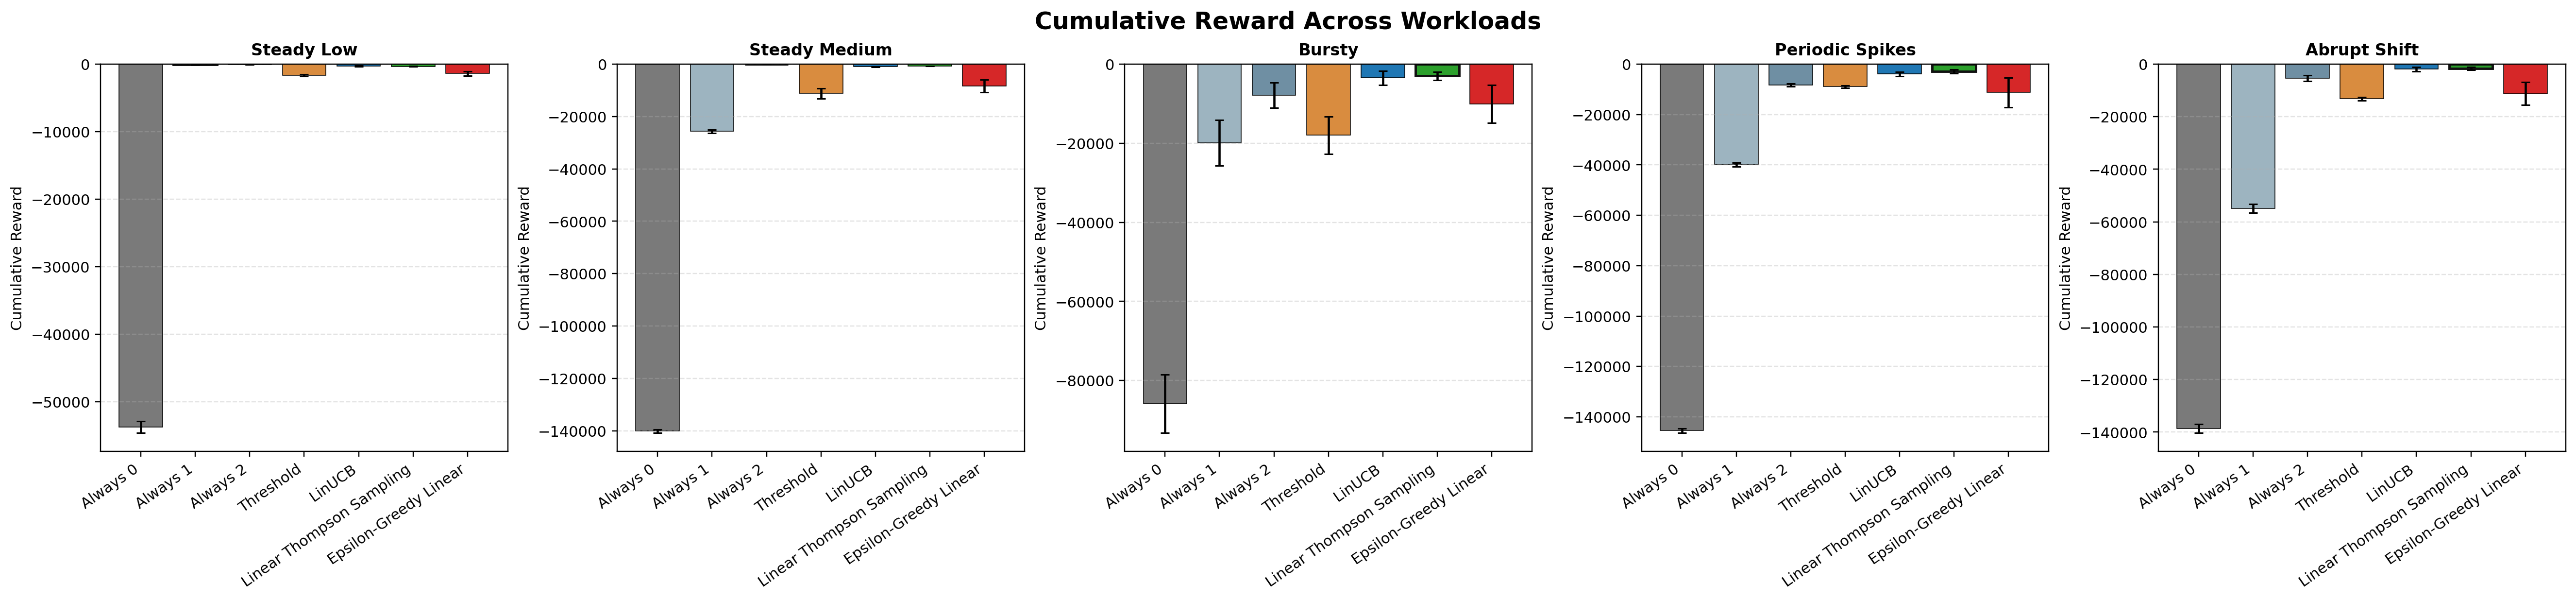
\includegraphics[width=\textwidth]{figure_1_cumulative_reward.png}
    \caption{Cumulative reward across all workloads. Higher (less negative) is better. Error bars show standard deviation over 3 seeds. LinUCB and LTS dominate on dynamic workloads.}
    \label{fig:reward}
\end{figure}

On the Steady Low workload, the simple Always\_1 baseline performs best (reward $= -52.8$) since low demand rarely requires more than one instance, and keeping one warm avoids all cold starts at minimal cost. Both LinUCB ($-278.5$) and LTS ($-327.2$) perform respectably but incur some unnecessary cost from over-provisioning during early exploration. This is expected behavior for learning algorithms and the gap would narrow with a longer horizon.

On all dynamic workloads, the adaptive policies dramatically outperform fixed baselines. On the Bursty workload, LinUCB achieves a reward of $-3{,}496$ versus $-7{,}870$ for Always\_2 (the best fixed policy), a 55.6\% improvement. On the Abrupt Shift workload, LTS achieves $-1{,}183$ compared to $-5{,}418$ for Always\_2, a 78.2\% improvement.

\subsection{Average Latency}

Figure~\ref{fig:latency} presents average latency results. The Always\_0 policy (no prewarming) consistently produces latencies exceeding 1{,}000~ms---nearly the full cold-start penalty---across all workloads. The bandit policies achieve latencies in the 127--133~ms range on dynamic workloads, close to the 120~ms base latency floor.

\begin{figure}[H]
    \centering
    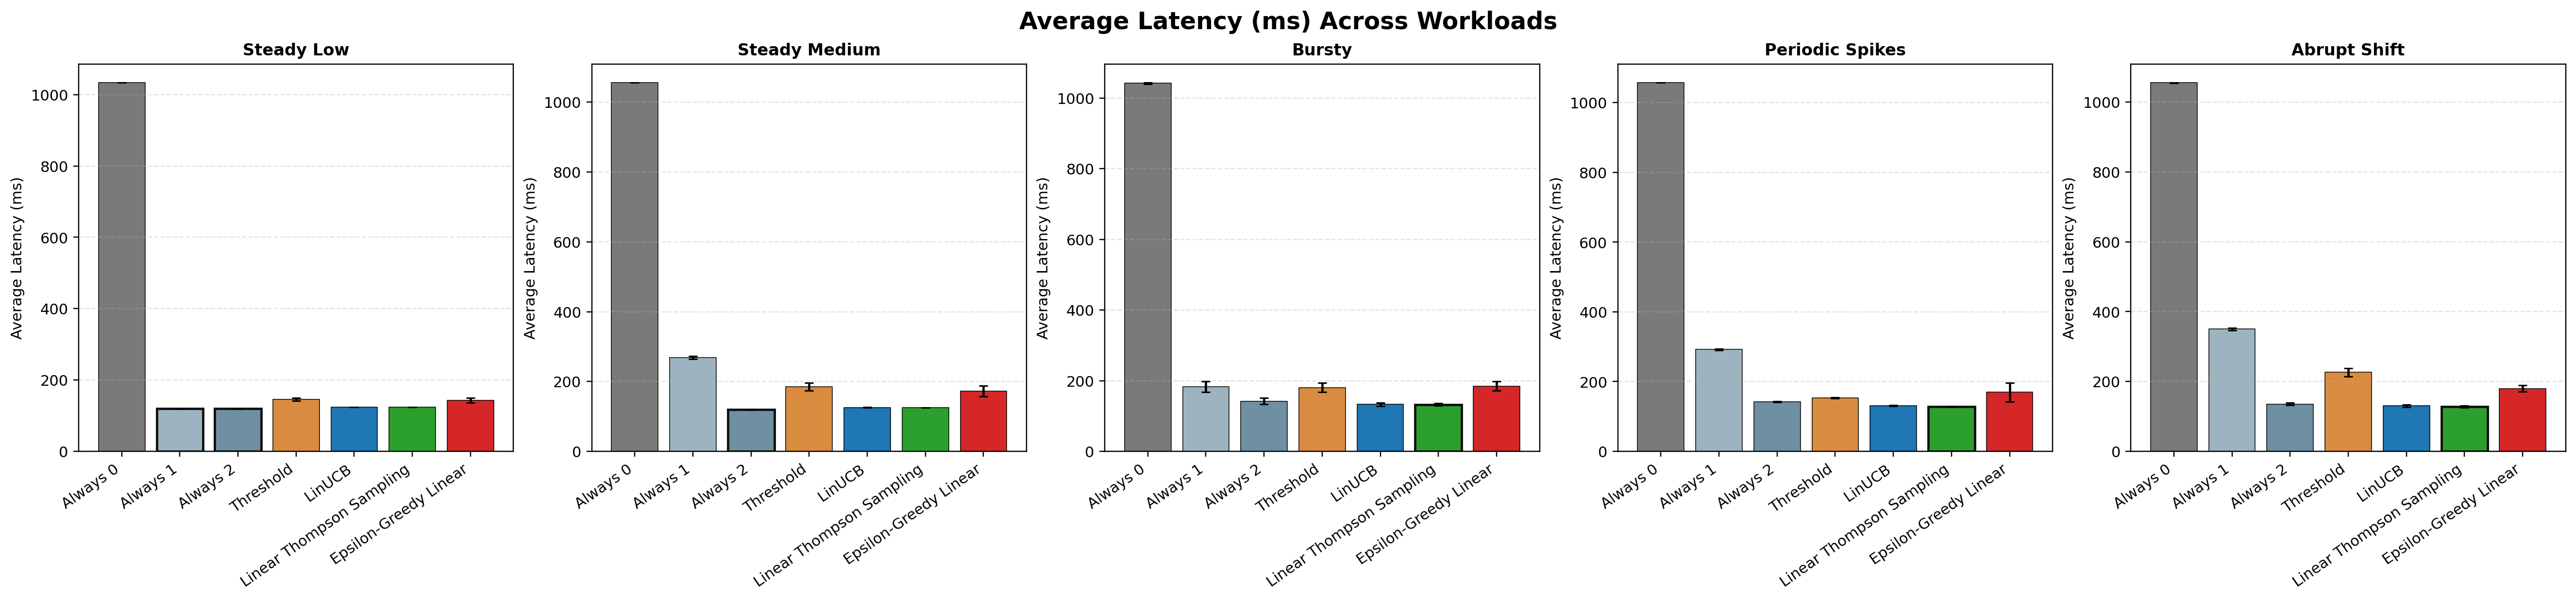
\includegraphics[width=\textwidth]{figure_2_avg_latency.png}
    \caption{Average latency (ms) across workloads. Lower is better. Bandit policies achieve near-optimal latency on all dynamic workloads.}
    \label{fig:latency}
\end{figure}

On the Abrupt Shift workload, the latency advantage is stark: LTS achieves 127.0~ms versus 350.2~ms for Always\_1 and 1{,}055.5~ms for Always\_0. The adaptive policies successfully detect the regime change at the midpoint and scale up prewarming accordingly.

\subsection{Cost Analysis}

Figure~\ref{fig:cost} shows total infrastructure cost. The bandit policies incur higher cost than minimal baselines (Always\_0, Always\_1) but achieve dramatically better performance. Importantly, LTS and LinUCB show cost discipline: on the Bursty workload, LinUCB incurs a cost of 166.3 while reducing cold starts from 6{,}973 (Always\_0) to 278---a 96\% reduction in cold starts for a cost that is still moderate.

\begin{figure}[H]
    \centering
    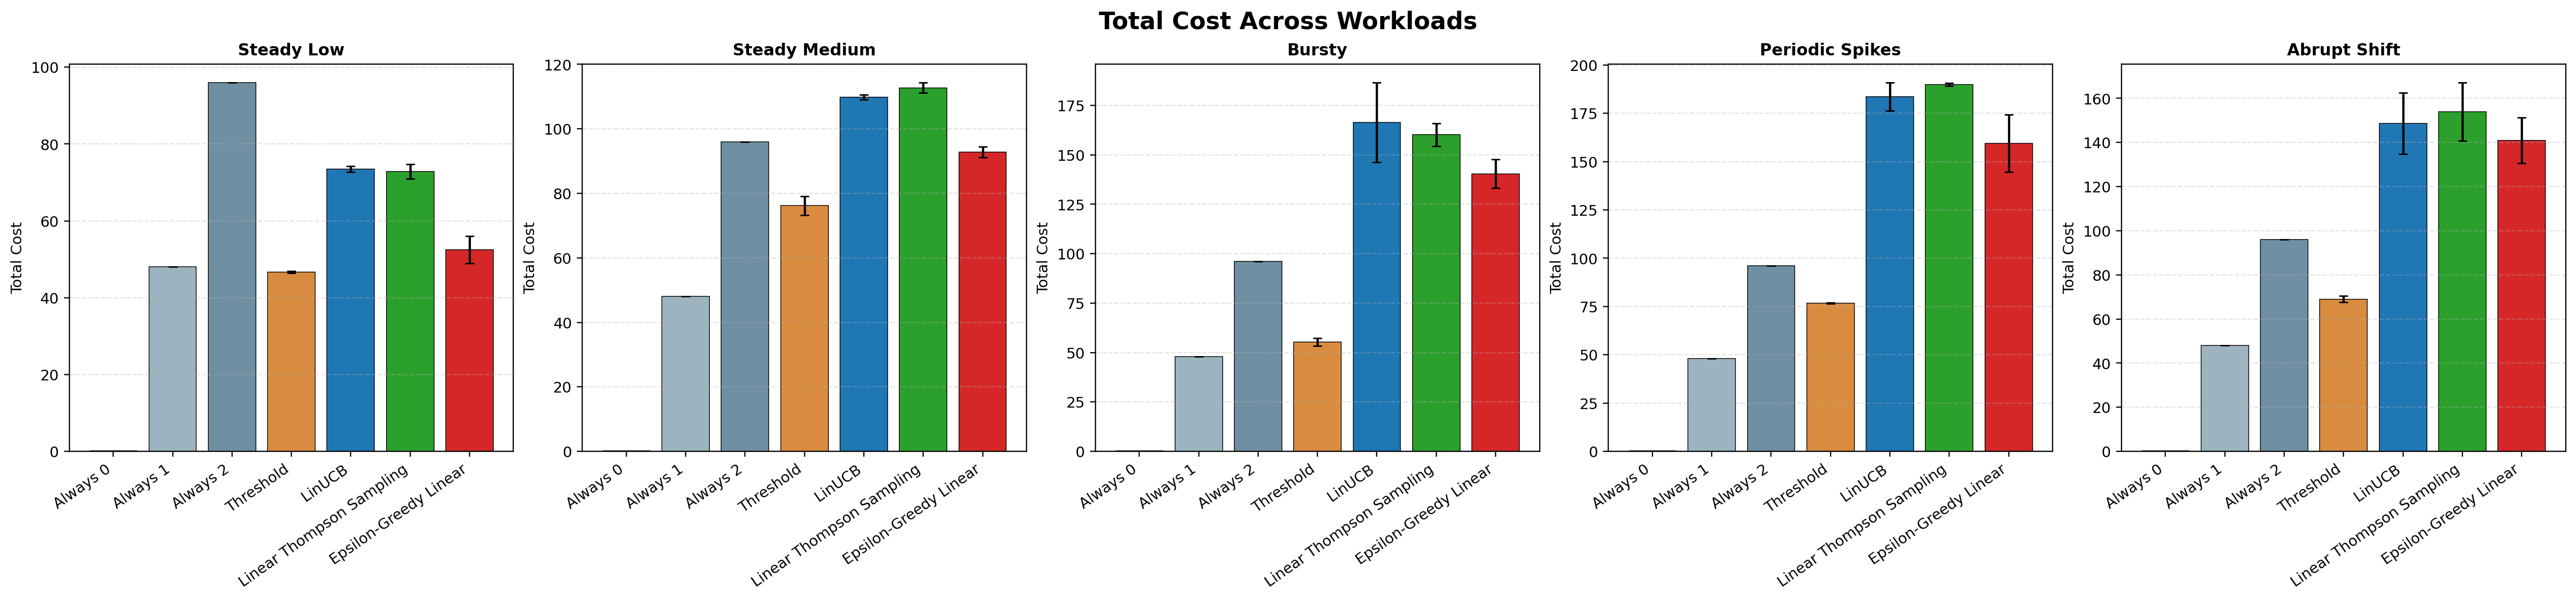
\includegraphics[width=\textwidth]{figure_3_total_cost.png}
    \caption{Total cost across workloads. The bandit policies spend more than minimal baselines but achieve substantially better latency and SLA compliance.}
    \label{fig:cost}
\end{figure}

\subsection{Detailed Results}

Table~\ref{tab:results} summarizes key metrics for the three most dynamic workloads, where the differences between policies are most pronounced.

\begin{table}[H]
\centering
\caption{Selected results on dynamic workloads (averaged over 3 seeds).}
\label{tab:results}
\small
\begin{tabular}{@{}llrrrrr@{}}
\toprule
\textbf{Workload} & \textbf{Policy} & \textbf{Reward} & \textbf{Latency (ms)} & \textbf{SLA Viol.} & \textbf{Cold Starts} & \textbf{Cost} \\
\midrule
Bursty     & LinUCB     & $-3{,}496$   & 133.0 & 1.18  & 278   & 166.3 \\
           & LTS        & $-3{,}676$   & 133.2 & 1.25  & 293   & 150.1 \\
           & Always\_2  & $-7{,}870$   & 141.9 & 2.73  & 635   & 96.0  \\
           & Always\_0  & $-85{,}850$  & 1041.8 & 30.06 & 6973 & 0.0   \\
\midrule
Periodic   & LTS        & $-2{,}908$   & 128.2 & 0.97  & 230   & 189.9 \\
           & LinUCB     & $-3{,}901$   & 131.5 & 1.32  & 312   & 183.6 \\
           & Always\_2  & $-8{,}300$   & 142.6 & 2.88  & 672   & 96.0  \\
           & Threshold  & $-8{,}954$   & 153.5 & 3.14  & 714   & 76.7  \\
\midrule
Abrupt     & LTS        & $-1{,}183$   & 127.0 & 0.38  & 86    & 159.2 \\
           & LinUCB     & $-1{,}939$   & 130.4 & 0.65  & 147   & 148.7 \\
           & Always\_2  & $-5{,}418$   & 135.6 & 1.90  & 424   & 96.0  \\
           & Always\_0  & $-138{,}673$ & 1055.5 & 48.40 & 11375 & 0.0  \\
\bottomrule
\end{tabular}
\end{table}

\subsection{Discussion}

\textbf{H1 is confirmed} on all non-trivial workloads. The contextual bandit policies achieve higher cumulative reward than every baseline on Steady Medium, Bursty, Periodic Spikes, and Abrupt Shift. On Steady Low, fixed policies are competitive because the workload is simple enough that a static choice (Always\_1) is near-optimal, and exploration overhead penalizes the learning algorithms slightly.

\textbf{H2 is confirmed.} The performance gap between adaptive and fixed policies widens substantially on dynamic workloads. On Steady Low, the best bandit (LinUCB at $-278$) is roughly 5$\times$ worse than Always\_1 ($-53$). On Abrupt Shift, the best bandit (LTS at $-1{,}183$) is 4.6$\times$ \emph{better} than the best fixed policy (Always\_2 at $-5{,}418$). This demonstrates that the value of adaptation scales with workload complexity.

\textbf{H3 is partially confirmed.} LTS and LinUCB consistently outperform Epsilon-Greedy Linear, often by large margins. For example, on Periodic Spikes, LTS achieves $-2{,}908$ versus $-11{,}254$ for Epsilon-Greedy---nearly a 4$\times$ improvement. The undirected exploration of epsilon-greedy wastes samples on poorly suited actions, whereas LTS and LinUCB concentrate exploration where uncertainty is highest.

Between LTS and LinUCB, LTS tends to perform slightly better on workloads with periodic or gradual structure (Periodic Spikes, Abrupt Shift), while LinUCB has a slight edge on the Bursty workload. This is consistent with the theoretical expectation that Thompson Sampling's stochastic exploration is more efficient in structured environments, while UCB's deterministic optimism is slightly more robust to random bursts.

% ============================================================
% 7. CONCLUSION AND FUTURE WORK
% ============================================================
\section{Conclusion and Future Work}

This project demonstrates that the serverless prewarming problem can be effectively addressed using contextual bandit methods. By framing instance prewarming as an online decision-making problem and leveraging recent workload context, our adaptive policies learn to balance latency, SLA compliance, and cost without requiring explicit demand forecasts.

Our key finding is that Linear Thompson Sampling and LinUCB consistently outperform static baselines on dynamic workloads, with improvements ranging from 55\% to 78\% in cumulative reward on the most challenging scenarios. The advantage is most pronounced precisely where it matters most: under bursty, periodic, and abruptly shifting demand patterns that fixed policies cannot handle.

Several directions for future work are promising. First, extending the action space to include finer-grained prewarming levels (e.g., 3, 5, 6 instances) or even continuous actions would allow more precise resource allocation. Second, incorporating non-linear models such as neural network--based bandits could capture more complex workload--reward relationships. Third, evaluating these policies on real-world serverless traces (e.g., the Azure Functions dataset from Shahrad et al.~\cite{shahrad2020}) would validate the simulation findings. Fourth, adding a non-stationarity detection mechanism could allow the agent to reset or discount old observations when a regime change is detected, potentially improving performance on abrupt shifts. Finally, extending the framework to multi-function serverless applications where prewarming decisions for different functions interact would address a more realistic deployment scenario.

% ============================================================
% REFERENCES
% ============================================================
\bibliographystyle{plain}

\begin{thebibliography}{11}

\bibitem{bermbach2020}
D.~Bermbach, A.-S. Karakaya, and S.~Buchholz.
\newblock Using application knowledge to reduce cold starts in FaaS services.
\newblock In \emph{Proceedings of the ACM Symposium on Applied Computing}, pages 134--143, 2020.

\bibitem{lin2020}
P.~Lin and H.~Khazaei.
\newblock Modeling and optimization of performance and cost of serverless applications.
\newblock \emph{IEEE Transactions on Parallel and Distributed Systems}, 32(3):615--632, 2020.

\bibitem{shahrad2020}
M.~Shahrad, R.~Fonseca, I.~Goiri, G.~Chaudhry, P.~Batum, J.~Cober, et~al.
\newblock Serverless in the wild: Characterizing and optimizing the serverless workload at a large cloud provider.
\newblock In \emph{USENIX ATC}, pages 205--218, 2020.

\bibitem{li2010}
L.~Li, W.~Chu, J.~Langford, and R.~E. Schapire.
\newblock A contextual-bandit approach to personalized news article recommendation.
\newblock In \emph{Proceedings of the 19th International Conference on World Wide Web}, pages 661--670, 2010.

\bibitem{agrawal2013}
S.~Agrawal and N.~Goyal.
\newblock Thompson sampling for contextual bandits with linear payoffs.
\newblock In \emph{Proceedings of the 30th International Conference on Machine Learning}, pages 127--135, 2013.

\bibitem{singhvi2021}
A.~Singhvi, A.~Balasubramanian, K.~Houck, M.~D. Shaikh, S.~Padmanabhan, and S.~Banerjee.
\newblock Atoll: A scalable low-latency serverless platform.
\newblock In \emph{ACM Symposium on Cloud Computing}, pages 138--152, 2021.

\bibitem{yemets2024}
K.~Yemets.
\newblock A time series forecasting approach to minimize cold start time in cloud-serverless platform.
\newblock Master's thesis, University of Engineering and Technology, 2024.

\bibitem{suleiman2024}
B.~Suleiman, M.~J. Alibasa, Y.-Y.~Chang, and A.~Anaissi.
\newblock Predictive auto-scaling: LSTM-based multi-step cloud workload prediction.
\newblock In \emph{ICSOC 2023 Workshops}, LNCS 14518, pages 3--18. Springer, 2024.

\bibitem{kyrychenko2025}
O.~Kyrychenko, S.~Ostapov, and O.~L. Kyrychenko.
\newblock Predictive autoscaling in AWS serverless by means of machine learning.
\newblock In \emph{CEUR Workshop Proceedings}, volume 3963, 2025.

\bibitem{flashserve2025}
FlashServe.
\newblock Cost-efficient serverless inference scheduling for large language models via tiered memory management and predictive autoscaling.
\newblock \emph{Preprints.org}, 2025.

\bibitem{chai2025}
X.~Chai, T.~Zhou, K.~Hu, J.~Tan, T.~Bie, A.~Shen, et~al.
\newblock Fork in the road: Reflections and optimizations for cold start latency in production serverless systems.
\newblock In \emph{19th USENIX Symposium on Operating Systems Design and Implementation (OSDI 25)}, pages 199--218, 2025.

\end{thebibliography}

\end{document}
